\documentclass[12pt]{article}
\usepackage{amsmath}
\usepackage{amssymb}
\usepackage{geometry}
\usepackage{enumerate}
\usepackage{natbib}
\usepackage{float}%稳定图片位置
\usepackage{graphicx}%画图
\usepackage[english]{babel}
\usepackage{a4wide}
\usepackage{indentfirst}%缩进
\usepackage{enumerate}%加序号
\usepackage{multirow}%合并行


\begin{document}
\newpage
\textbf{Problem 2.(a)}
\begin{figure}[H]
\centering
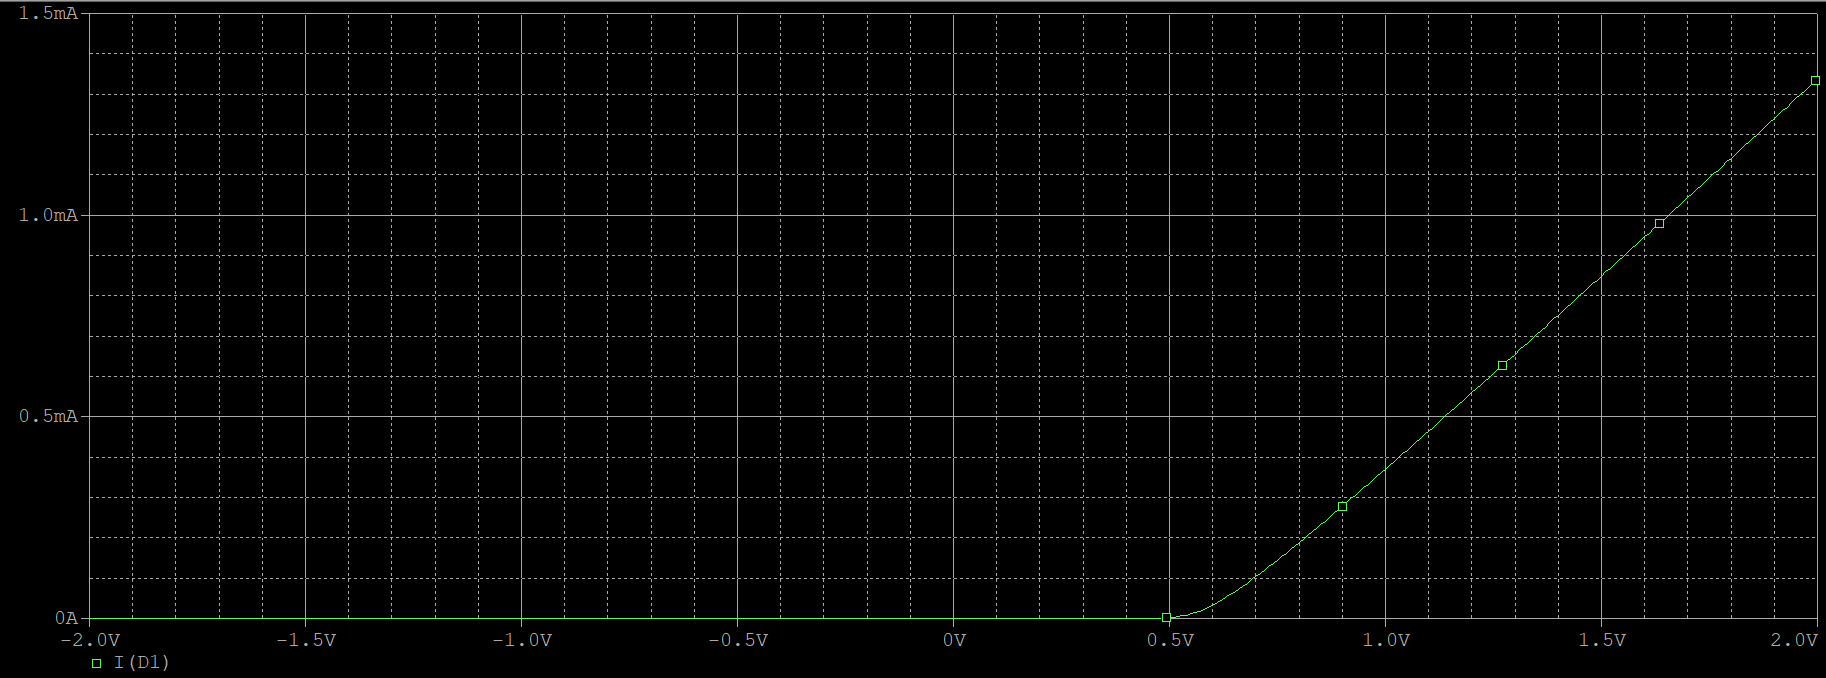
\includegraphics[scale=0.25]{P1.png}
\end{figure}
According to diode's voltage-current relation $$I_D=I_s(e^\frac{qV_a}{kT}-1)$$ and the current relation $$V=V_a+1000I_d=1000I_d+\frac{kT}{q}\ln(\frac{I_d}{I_s}+1)$$
\par Since $\frac{kt}{q}=0.0258$ so the second part of V can be omitted and as a result $I_d=\frac{V}{1000}$
so the current is increasing linearly.
\\\
\par \textbf{Problem 2.(b)}
\begin{figure}[H]
\centering
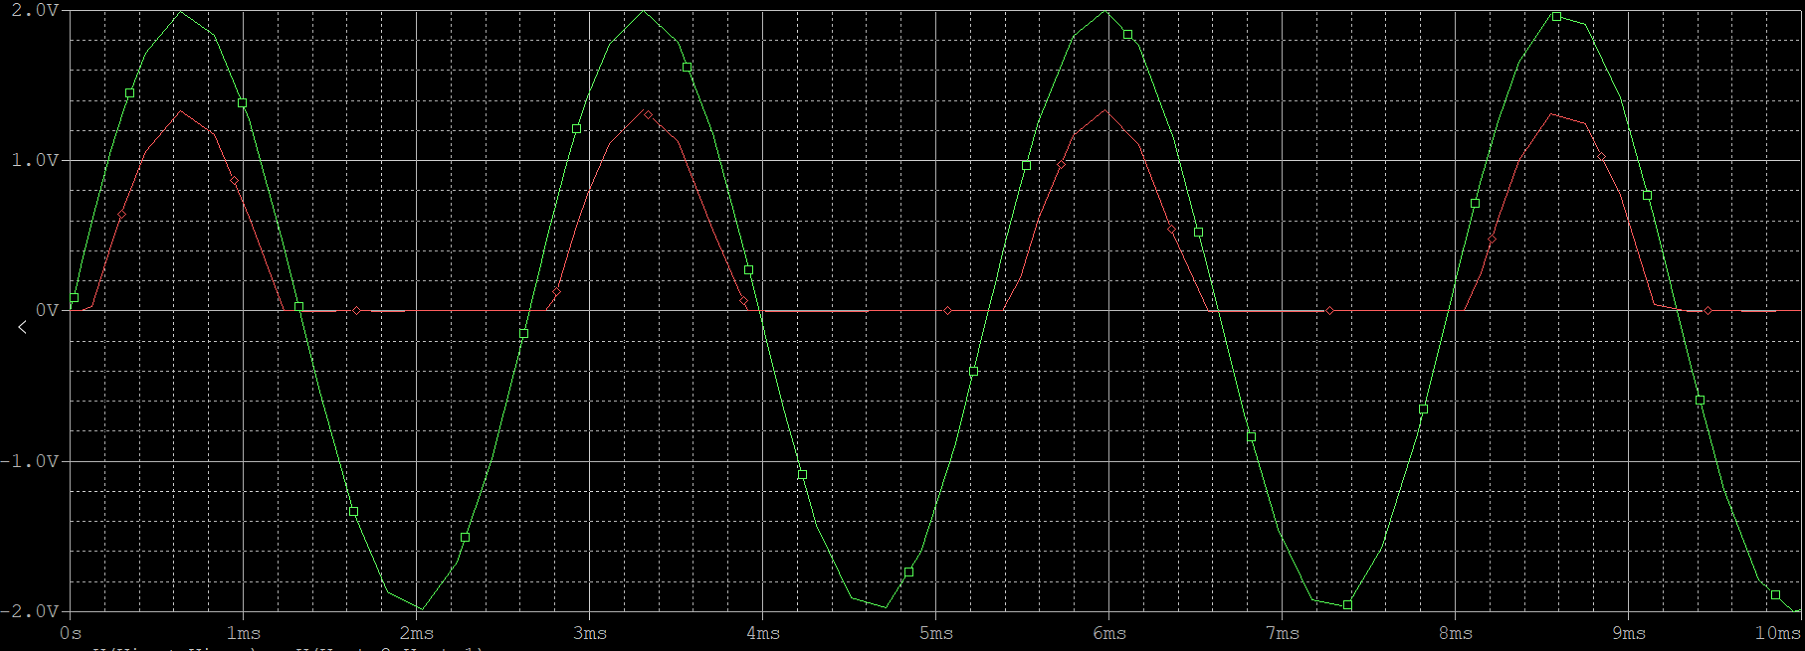
\includegraphics[scale=0.25]{P2.png}
\end{figure}
The green line represents for the $V_{in}$ and the red line represents for the $V_{out}$, so the circuit can stop the current when the input voltage is negative and decrease the voltage for the resistor when the input voltage is positive.
\end{document}